\section{引言}

将大型语言模型(LLMs,~\citealt{brown2020language,chowdhery2023palm, touvron2023llama,achiam2023gpt})与人类伦理标准和实践预期对齐,对于防止意外后果并确保人工智能对社会的积极贡献至关重要。传统的对齐方法,如监督微调(SFT)和基于人类反馈的强化学习(RLHF)~\cite{bai2022constitutional, ouyang2022training},资源消耗大,并且需要大量的人类监督,限制了它们的可扩展性和实用性。随着LLM变得更加复杂和广泛应用,对成本效益高、标注效率高、快速适应的对齐策略的需求变得越来越迫切。

\begin{figure}
    \centering
    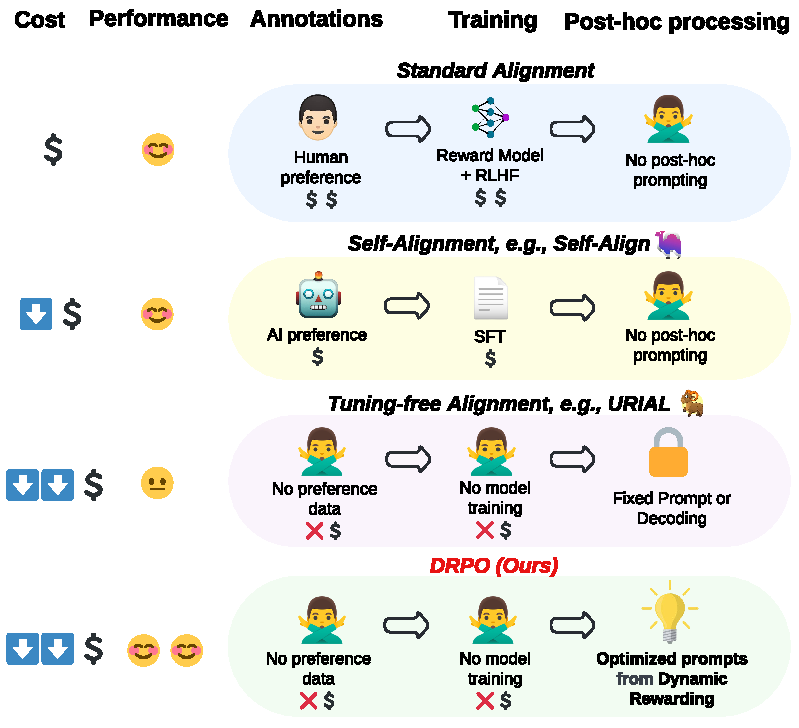
\includegraphics[width=1\linewidth]{images/DRPO_comparison.pdf}
    \vspace{-18pt}
    \caption{与其他LLM对齐范式的对比。 \ours结合了自我对齐和无需调优对齐的优点,能够实现自我改进和高效的成本效益,无需人工监督或额外的模型训练。}
    \vspace{-22pt}
    \label{fig:paradigm_comparison}
\end{figure}

自我对齐旨在通过利用模型本身来改善LLM对齐;例如,通过用模型生成的反馈代替人工反馈~\cite{lee2023rlaif},合成偏好数据~\cite{kim2023aligning, sun2024principle},或自我批评~\cite{bai2022constitutional}。尽管有这些进展,这些方法仍然需要大量资源,包括成本高昂且不稳定的RLHF调优,以及某些程度的人工监督,例如精心策划的对齐规则或上下文学习(ICL)提示~\cite{sun2024principle}。另一方面,如图~\ref{fig:paradigm_comparison}所示,最近的研究重点是无需调优的对齐,优先考虑极高的效率,而不需要承担任何调优成本。这些方法包括基于解码的对齐技术~\cite{li2023rain, wang2024inferaligner}或ICL对齐~\cite{han2023context, Lin2024ReAlign, zhao2024context}。然而,这些无需调优的方法通常是静态的(例如,依赖于固定的提示或奖励函数),因此缺乏适应性和自我改进能力,以实现更好的对齐。

为了结合这两种范式的优点,本文提出了\ours,动态奖励与提示优化(Dynamic Rewarding with Prompt Optimization),一种新的无需调优的LLM自我对齐方法。 \ours从近期对齐研究中的两个关键见解中汲取灵感。首先,表面对齐假设~\cite{zhou2024lima}表明,通过轻量级的调优或简单的提示,LLM可以有效地进行对齐~\cite{Lin2024ReAlign, zhao2024context}。其次,RLHF中的奖励模型往往对分布外样本的泛化能力较差~\cite{burns2023weak},而LLM因其出色的泛化能力,可以提供更有效的奖励和反馈来进行对齐。基于这些见解,\ours构建在基于搜索的提示优化(PO)框架之上~\cite{pryzant2023automatic, hao2023reasoning, wang2023promptagent},该框架使得LLM能够自我修正并自动生成详细的对齐指令,从而更加有效地引导模型行为,而无需依赖于任何人工偏好或模型训练。

\ours的核心创新在于其\textit{动态奖励}机制,与优化框架集成在一起。该机制允许基于LLM的奖励根据具体查询动态调整,有助于识别和解决模型的对齐盲点。例如,如果一个LLM因知识过时而假装回答一个需要最新新闻的问题,它的“知识限制”奖励将很低,并且对齐提示将相应地更新。我们将这种新方法应用于自动生成系统提示和ICL示例中的响应,证明其在提升对齐方面极为有效。

我们对8个近期的LLM进行了全面的实验,使用了标准的对齐基准\texttt{just-eval-instruct},该基准由多个对齐数据集中的问题组成。我们的结果表明,\ours能够有效地对齐基本模型和SFT/RLHF调优模型。特别地,\ours显著增强了基本模型,使其表现超过了经过SFT/RLHF调优的模型。 \ours还能够进一步提升SFT/RLHF调优模型,突显了它与其他基于调优的对齐技术的兼容性。此外,我们自动优化的提示在效果上远超由人类专家策划的提示。

\begin{figure}
    \centering
    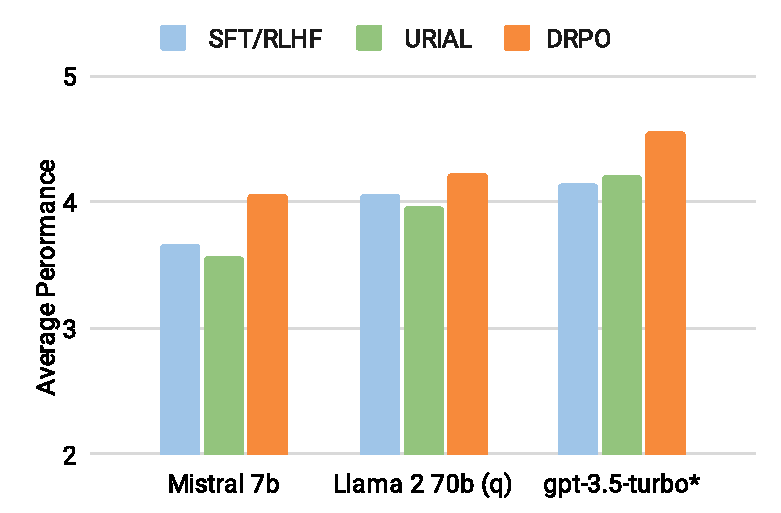
\includegraphics[width=1.0\linewidth]{images/method_comparison_column_chart_white_bg.pdf}
    \vspace{-15pt}
    \caption{与其他对齐方法(包括RLHF和URIAL~\cite{Lin2024ReAlign})的对比。 \ours在多个LLM上始终优于这两种基线。
    请注意,我们无法访问\texttt{gpt-3.5-turbo}基本模型;因此,\ours和URIAL直接应用于其RLHF调优版本。}
    \label{fig:overall_comparison_chart}
    \vspace{-15pt}
\end{figure}
